\documentclass[12pt]{beamer}

\usetheme{Malmoe}
\usepackage[utf8]{inputenc}
\usepackage{graphicx}
\usepackage{xcolor}
\usepackage{wrapfig} % texlive-latex-extra package
\usepackage{underscore}

\definecolor{Cyan}{RGB}{0,141,184}
\setbeamercolor{structure}{fg=Cyan}

\setbeamerfont{title}{series=\bfseries,parent=structure}
\setbeamerfont{subtitle}{size=\normalsize,series=\bfseries,parent=structure}
\setbeamerfont{author}{size=\scriptsize,series=\bfseries,parent=structure}
\setbeamerfont{institute}{size=\scriptsize,series=\bfseries,parent=structure}
\setbeamerfont{date}{size=\scriptsize,series=\bfseries,parent=structure}

\title{GIS.lab}
\subtitle{rapid GIS office deployment}
\author{Ivan Minčík (imincik)}
%\setbeamercovered{transparent} 
%\setbeamertemplate{navigation symbols}{} 
%\logo{} 
\institute{FOSS4G-Europe 2014, Bremen}
\date{} 
%\subject{}


\begin{document}

\begin{frame}
	\titlepage
\end{frame}


\section{Introduction}
\begin{frame}
	\begin{center}
		\LARGE\textbf{Introduction}	
	\end{center}
\end{frame}


\begin{frame}{What is GIS.lab ?}
	\begin{itemize}[<+->]
		\item NOT a single application
		\item comprehensive GIS infrastructure
		\item suitable for small and middle size deployment
		\item Open Source software
	\end{itemize}
\end{frame}


\begin{frame}{Goals}
	\begin{itemize}[<+->]
		\item self containing and independent system
		\item automatic deployment and management - plug-and-play
		\item zero maintenance costs
		\item prepared for use in LAN (server and desktop clients)
		\item prepared for use in data center or cloud (server)
		\item stable GIS software stack with maintenance patches
		\item good extensibility
		\item rapid failure recovery	
		\item very cheap
		\item small office server must fit in a pocket
	\end{itemize}
\end{frame}


\begin{frame}{GIS.lab architecture}
	\begin{itemize}
		\item automatically installed GIS.lab server
		\item network booting, plug-and-play GIS.lab client machines
	\end{itemize}
	\begin{center}
		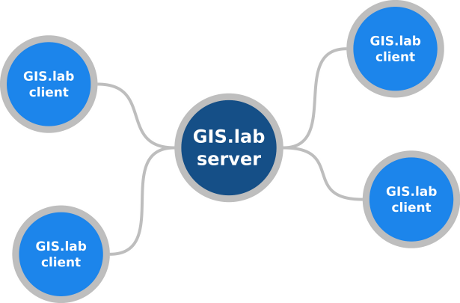
\includegraphics[keepaspectratio=true,height=0.6\textheight]{images/gislab-architecture.png}
	\end{center}
\end{frame}


\begin{frame}{Features}
	\begin{itemize}[<+->]
		\item data storage and sharing (files, GeoDB)
		\item office productivity suite (text, images, video, chat)
		\item GIS data processing and analysis
		\item GIS project publishing on web
	\end{itemize}
\end{frame}


\begin{frame}{Development}
	\textbf{Versions}
	\begin{itemize}
		\item currently preparing for 0.4 release
		\item general production release 1.0 in end of 2014
	\end{itemize}

	\textbf{Authors}
	\begin{itemize}
		\item Marcel Dancák
		\item Ivan Minčík
	\end{itemize}

	\textbf{Sponsor}
	\begin{itemize}
		\item GISTA s.r.o.
	\end{itemize}
\end{frame}


\section{Installation in LAN}
\begin{frame}
	\begin{center}
		\LARGE\textbf{Installation in LAN}	
	\end{center}
\end{frame}


\begin{frame}{Requirements}
	\textbf{Server}
	\begin{itemize}
		\item single machine with Linux, Mac OX or Windows installed
	\end{itemize}
	
	\textbf{Client}
	\begin{itemize}
		\item multiple machines with any \textbf{or} no OS installed
	\end{itemize}
\end{frame}


\begin{frame}{Hard way}
	\textbf{Install dependencies}
	\begin{itemize}
		\item install VirtualBox, Vagrant, Git (optional)
	\end{itemize}

	\textbf{Install GIS.lab}
	\begin{itemize}
		\item \$ vagrant box add precise32-canonical http:// ...
		\item download installation ZIP \textbf{or} \$ git clone ...
		\item \$ vagrant up
	\end{itemize}
	\begin{flushleft}
		\textbf{\textcolor{Cyan}{25} minutes} \\
		\textbf{\textcolor{Cyan}{0} EUR} \\
	\end{flushleft}
\end{frame}


\begin{frame}{Easy way - GIS.lab Unit}
	\begin{minipage}[\textheight]{\textwidth}
	\begin{columns}[T]
		\begin{column}{0.5\textwidth}
			\vspace{0.2\textheight}
			Plug-and-play
			\begin{flushleft}
				\textbf{\textcolor{Cyan}{5} minutes} \\
				\textbf{\textcolor{Cyan}{450} EUR} \\
			\end{flushleft}
		\end{column}
		\begin{column}{0.5\textwidth}
			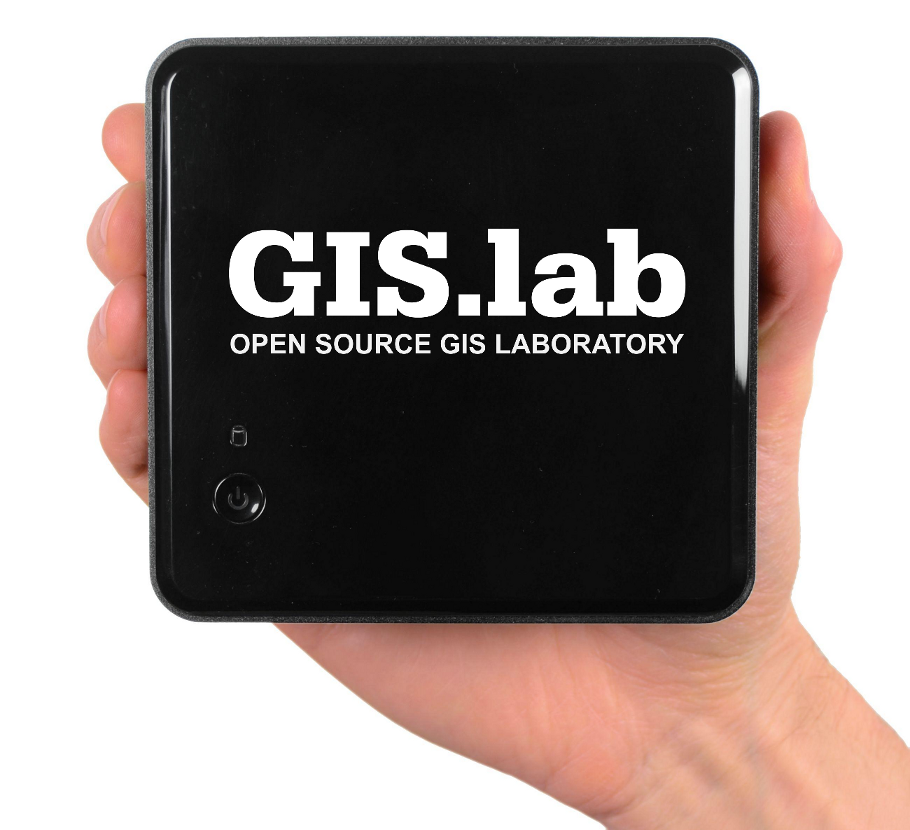
\includegraphics[keepaspectratio=true,width=\textwidth]{images/gislab-unit.png}
		\end{column}
	\end{columns}
	\end{minipage}
\end{frame}


\section{GIS.lab client}
\begin{frame}
	\begin{center}
		\LARGE\textbf{GIS.lab client}
	\end{center}
\end{frame}


\begin{frame}{Client modes}
	\textbf{Physical client}
	\begin{itemize}
		\item best performance - using all power of physical hardware
		\item original OS is temporary not available 
	\end{itemize}
	\begin{center}
		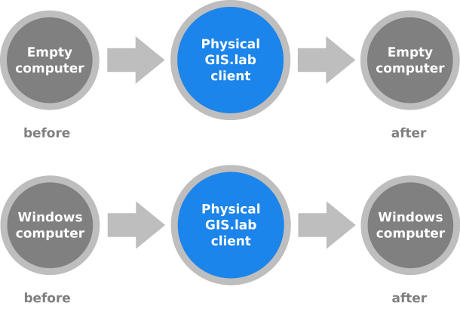
\includegraphics[keepaspectratio=true,height=0.6\textheight]{images/schema-physical-client.png}
	\end{center}
\end{frame}


\begin{frame}{Client modes}
	\textbf{Virtual client}
	\begin{itemize}
		\item lower performance - using all power of virtual machine
		\item original machine OS and GIS.lab client run side-by-side
	\end{itemize}
	\begin{center}
		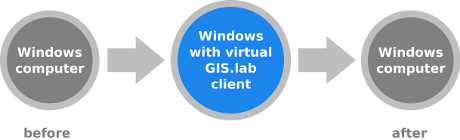
\includegraphics[keepaspectratio=true,height=0.4\textheight]{images/schema-virtual-client.png}
	\end{center}
\end{frame}


\begin{frame}{Client modes}
	\textbf{Third party clients}
	\begin{itemize}
		\item can use file or database storage
		\item can use WMS or WFS 
		\item can browse GIS project via Internet browser
	\end{itemize}
\end{frame}


\begin{frame}{Physical client configuration}
	\begin{itemize}
		\item enable 'legacy' boot and 'boot manager' in BIOS
		\item boot from LAN (PXE) in boot manager dialog (F12)
	\end{itemize}
	\begin{center}
		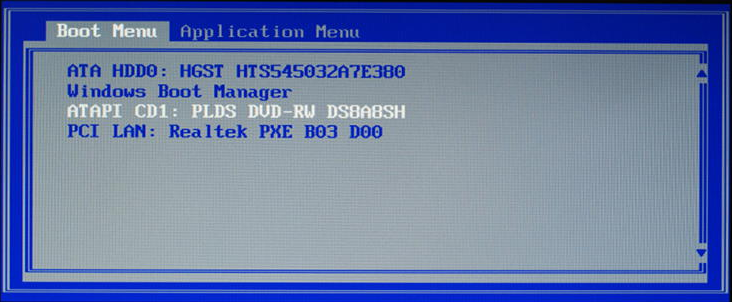
\includegraphics[keepaspectratio=true,height=0.6\textheight]{images/real-world-example/client-physical-configuration.png}
	\end{center}
\end{frame}


\begin{frame}{Virtual client configuration}
	\begin{itemize}
		\item create new VirtualBox machine with no hard drive
		\item configure virtual machine to boot from network
	\end{itemize}
	\begin{center}
		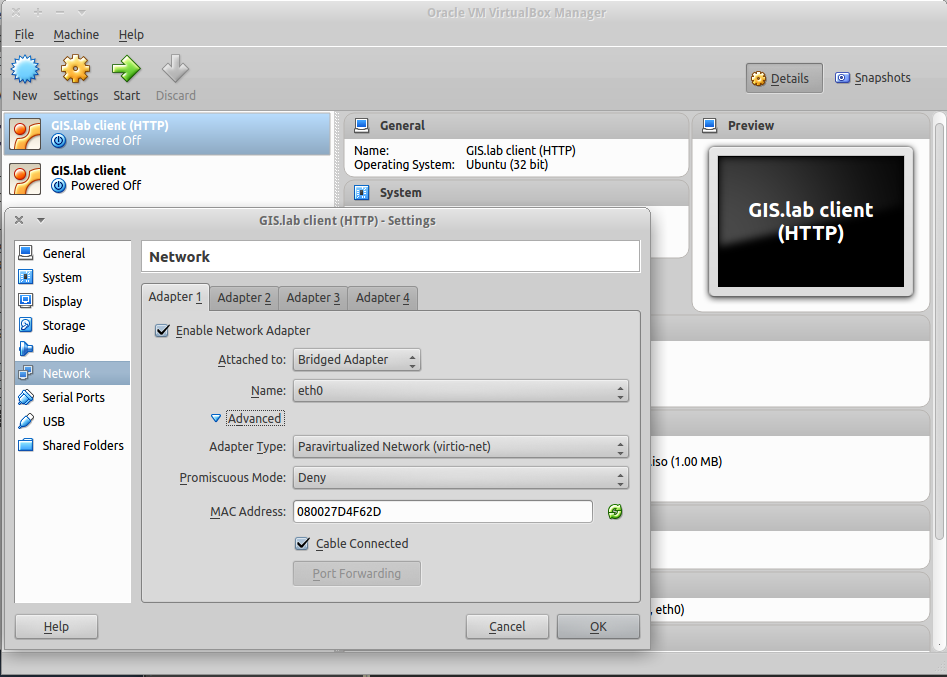
\includegraphics[keepaspectratio=true,height=0.6\textheight]{images/real-world-example/client-virtualbox-configuration.png}
	\end{center}
\end{frame}


\begin{frame}{Client launch}
	\begin{center}
		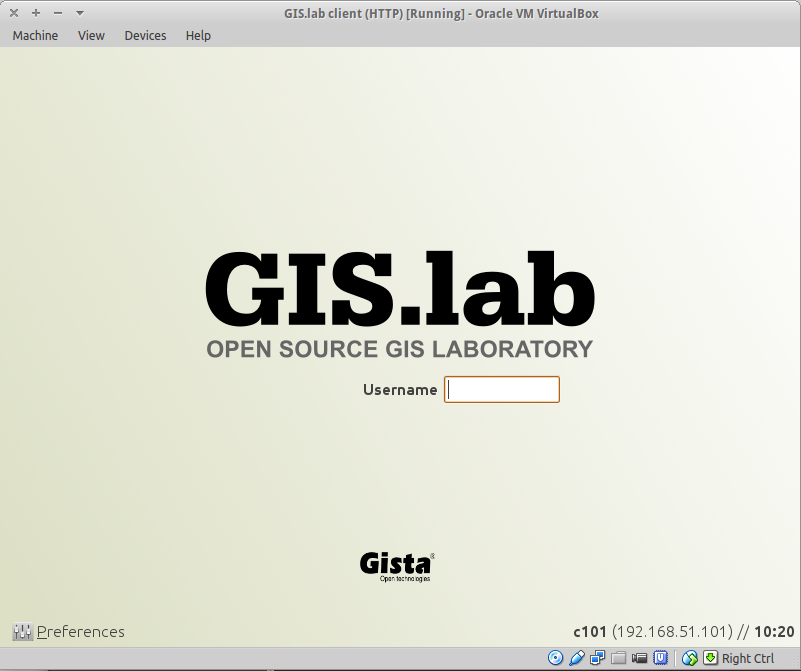
\includegraphics[keepaspectratio=true,height=0.7\textheight]{images/real-world-example/client-login.png}
	\end{center}
\end{frame}


\begin{frame}{Client desktop environment}
	\begin{center}
		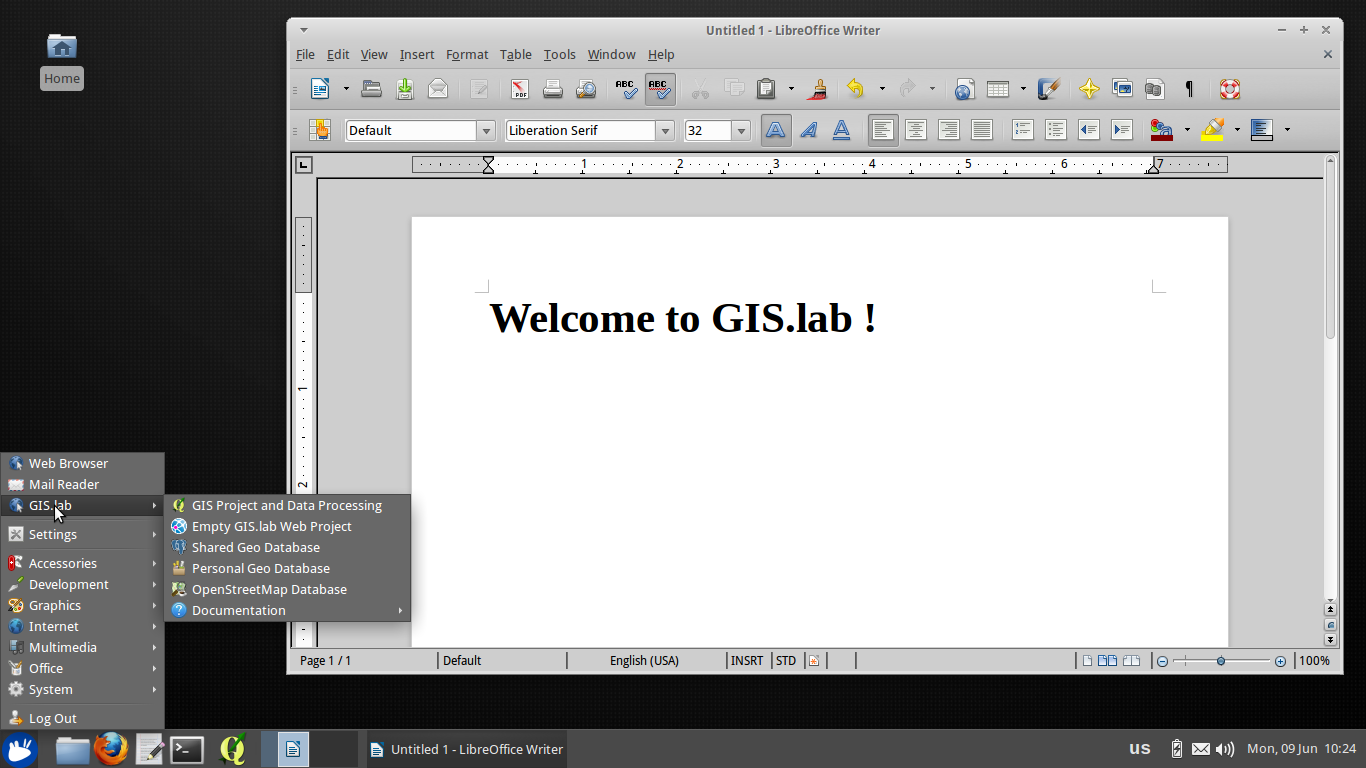
\includegraphics[keepaspectratio=true,height=0.7\textheight]{images/real-world-example/client-desktop-libreoffice.png}
	\end{center}
\end{frame}


\section{GIS project}
\begin{frame}
	\begin{center}
		\LARGE\textbf{Real world example}\normalsize

		\textbf{Map of Central Europe}
	\end{center}
\end{frame}


\begin{frame}{Spatial DB creation}
	\begin{itemize}
		\item create new SpatiaLite DB in SpatiaLite GUI
	\end{itemize}
	\begin{center}
		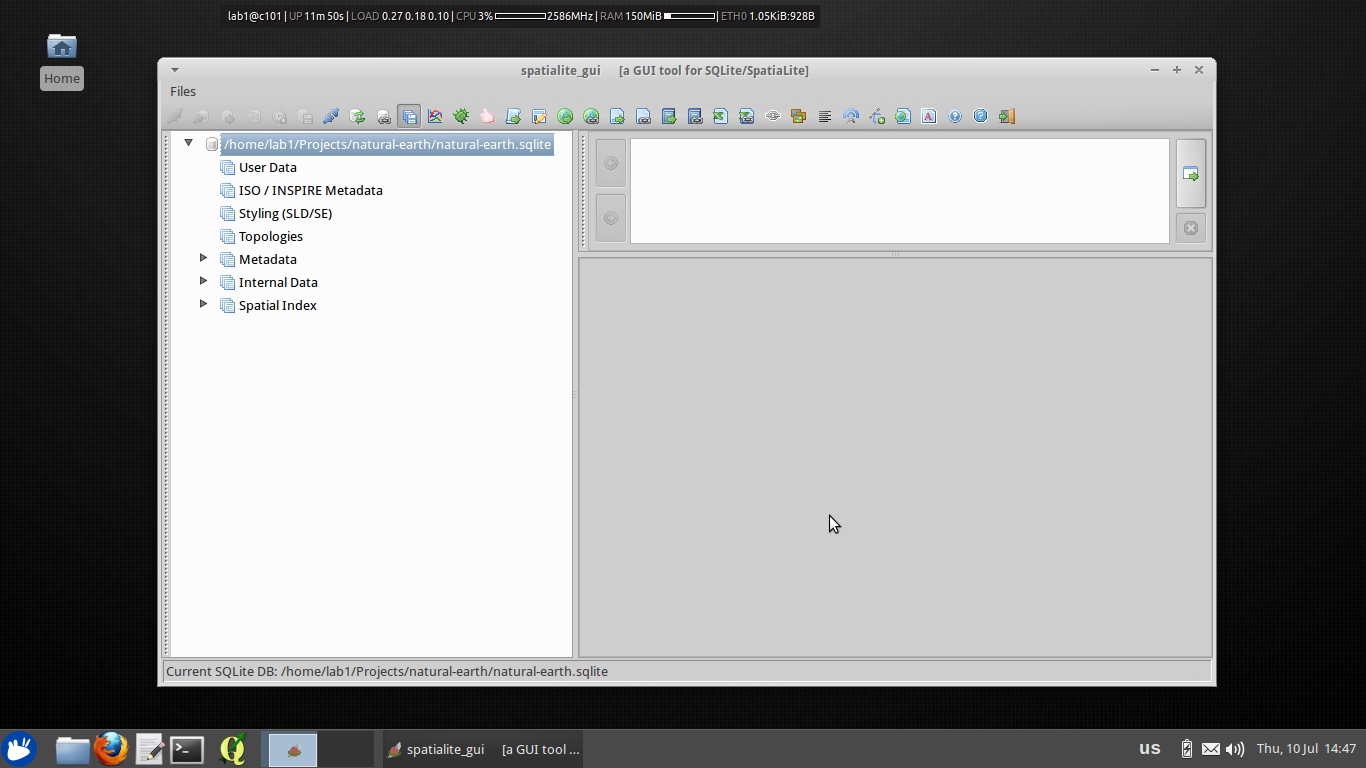
\includegraphics[keepaspectratio=true,height=0.7\textheight]{images/rapid-gis-deployment/project-create-db.png}
	\end{center}
\end{frame}


\begin{frame}{Data import}
	\begin{itemize}
		\item inspect data in QGIS
		\item import layers to Spatialite DB using DB Manager plugin
	\end{itemize}
	\begin{center}
		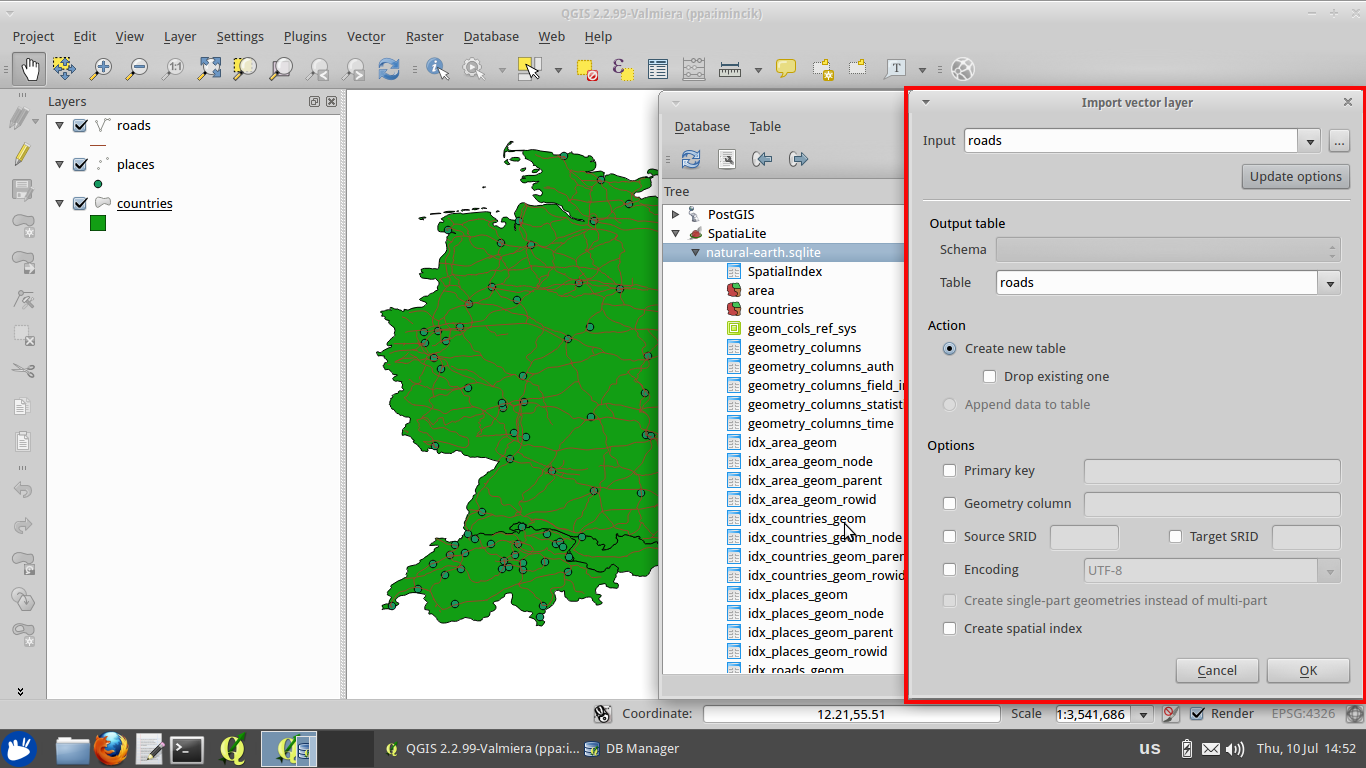
\includegraphics[keepaspectratio=true,height=0.6\textheight]{images/rapid-gis-deployment/project-db-import-layers.png}
	\end{center}
\end{frame}


\begin{frame}{GIS project creation}
	\begin{itemize}
		\item load imported layers back from SpatiaLite DB to QGIS
	\end{itemize}
	\begin{center}
		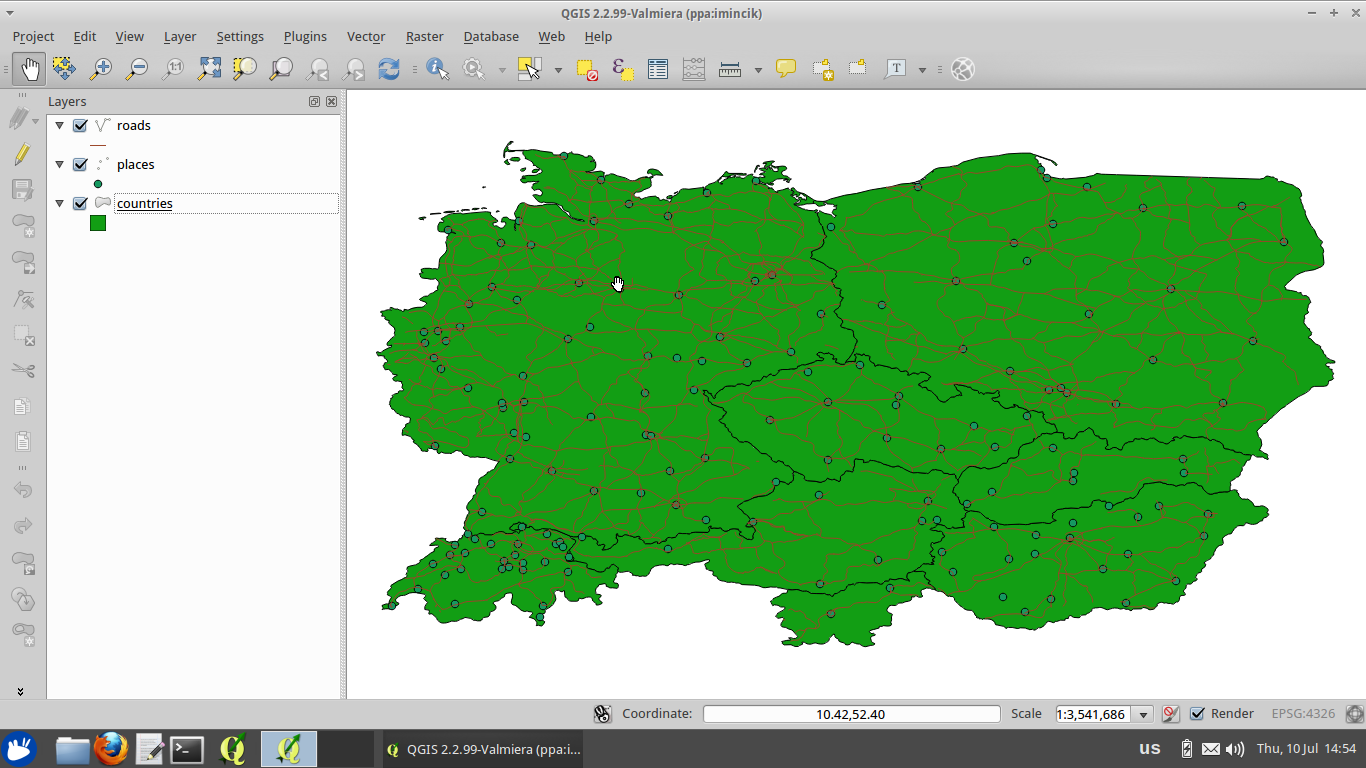
\includegraphics[keepaspectratio=true,height=0.6\textheight]{images/rapid-gis-deployment/project-db-load-layers.png}
	\end{center}
\end{frame}


\begin{frame}{TOC structure}
	\begin{itemize}
		\item create layer groups
		\item rename layers and move to corresponding groups
	\end{itemize}
	\begin{center}
		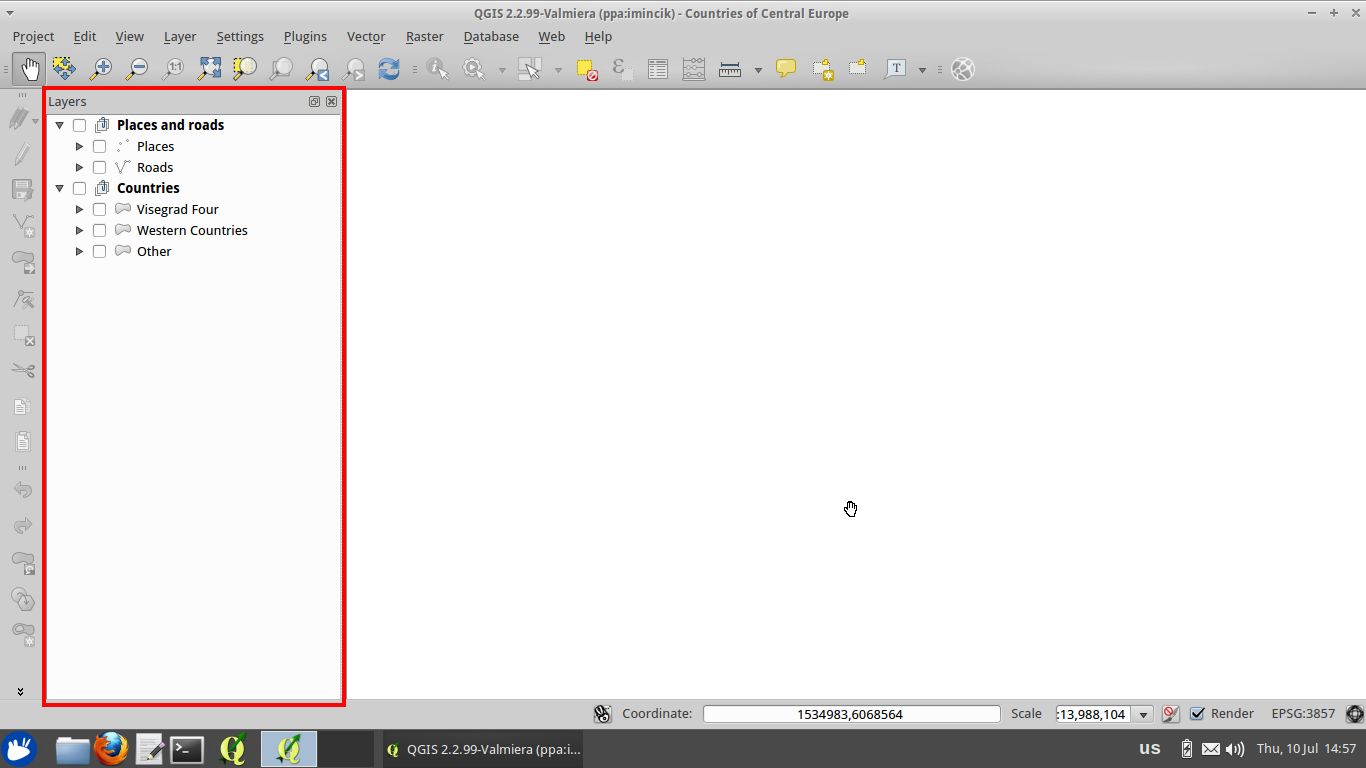
\includegraphics[keepaspectratio=true,height=0.6\textheight]{images/rapid-gis-deployment/project-create-toc-structure.png}
	\end{center}
\end{frame}


\begin{frame}{Layers styling}
	\begin{itemize}
		\item set styles and map symbols to each layer
		\item set layer style by attribute values
	\end{itemize}
	\begin{center}
		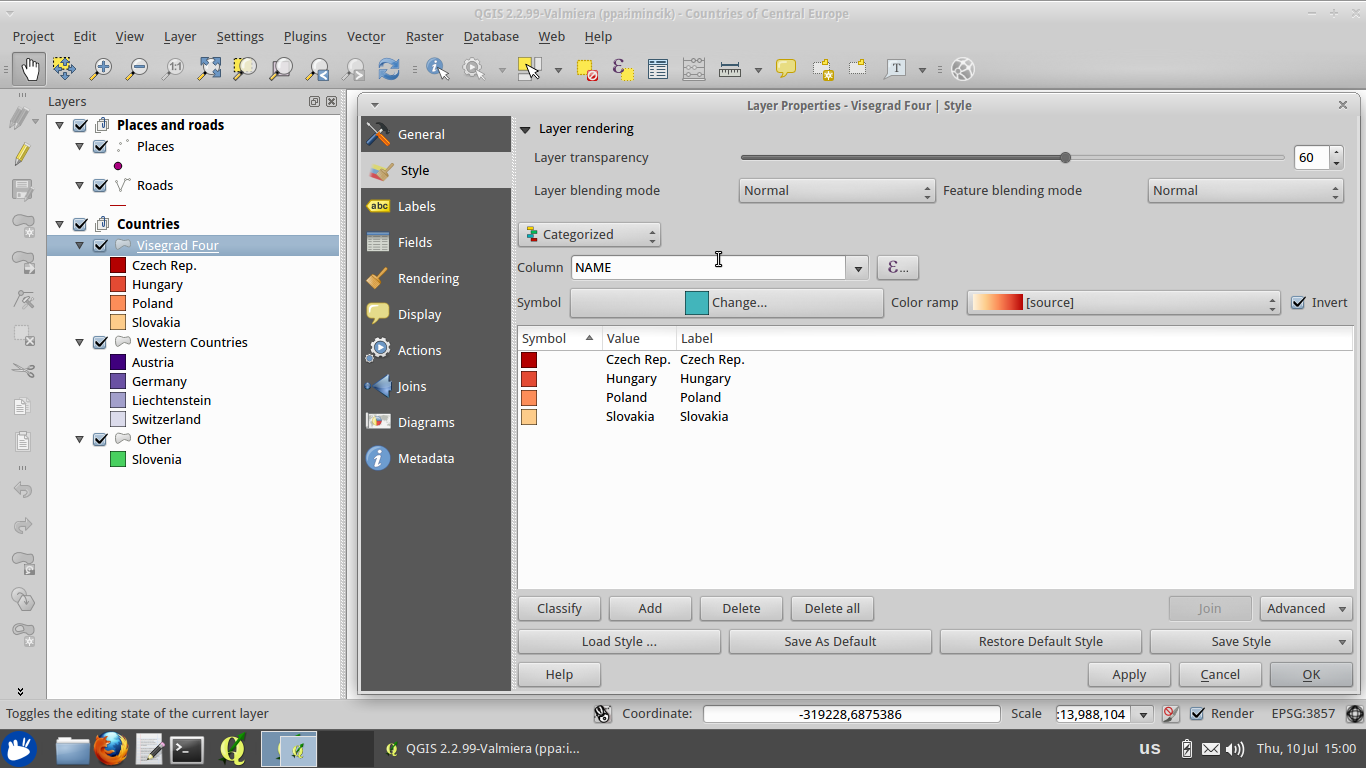
\includegraphics[keepaspectratio=true,height=0.6\textheight]{images/rapid-gis-deployment/project-layer-style.png}
	\end{center}
\end{frame}


\begin{frame}{Layers styling}
	\begin{center}
		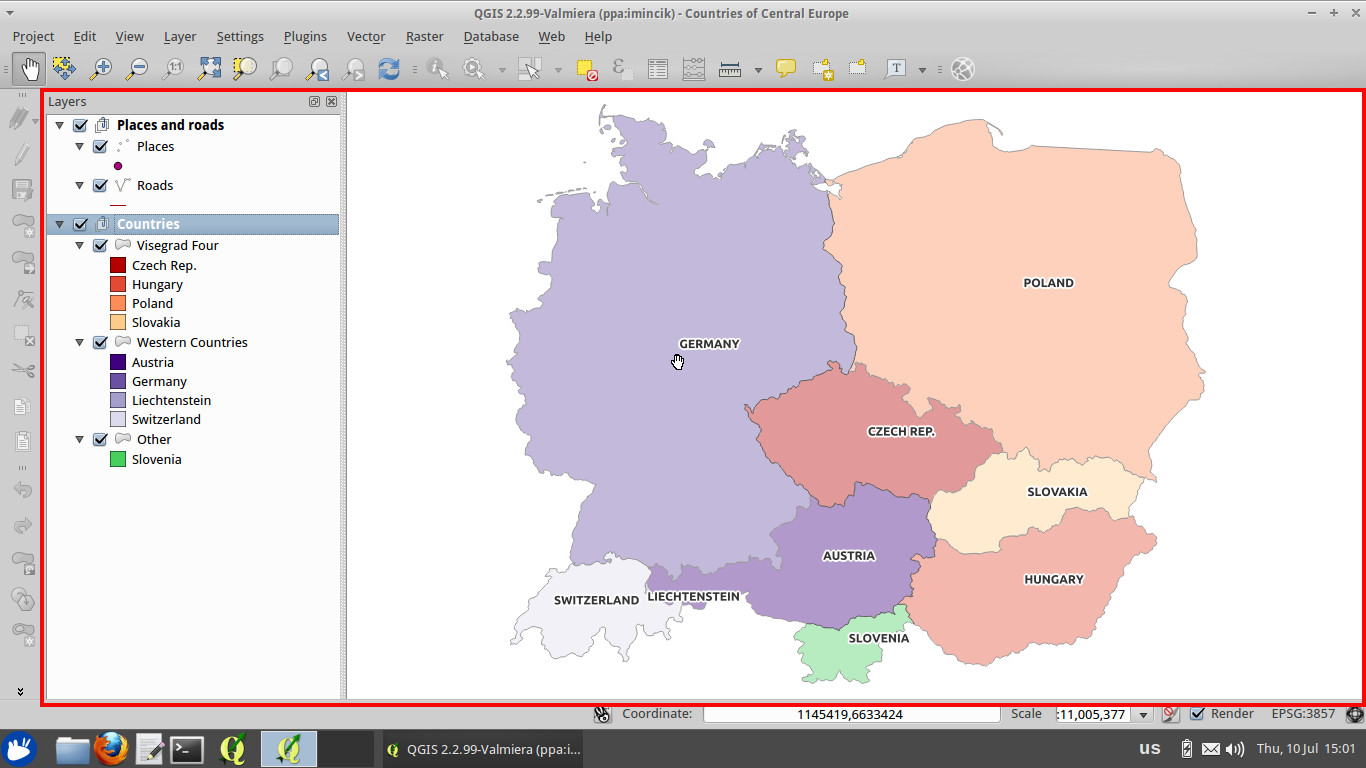
\includegraphics[keepaspectratio=true,height=0.6\textheight]{images/rapid-gis-deployment/project-layer-style-ready.png}
	\end{center}
\end{frame}


\begin{frame}{Attributes}
	\begin{itemize}
		\item set human names to attribute fields
		\item create attribute table form
	\end{itemize}
	\begin{center}
		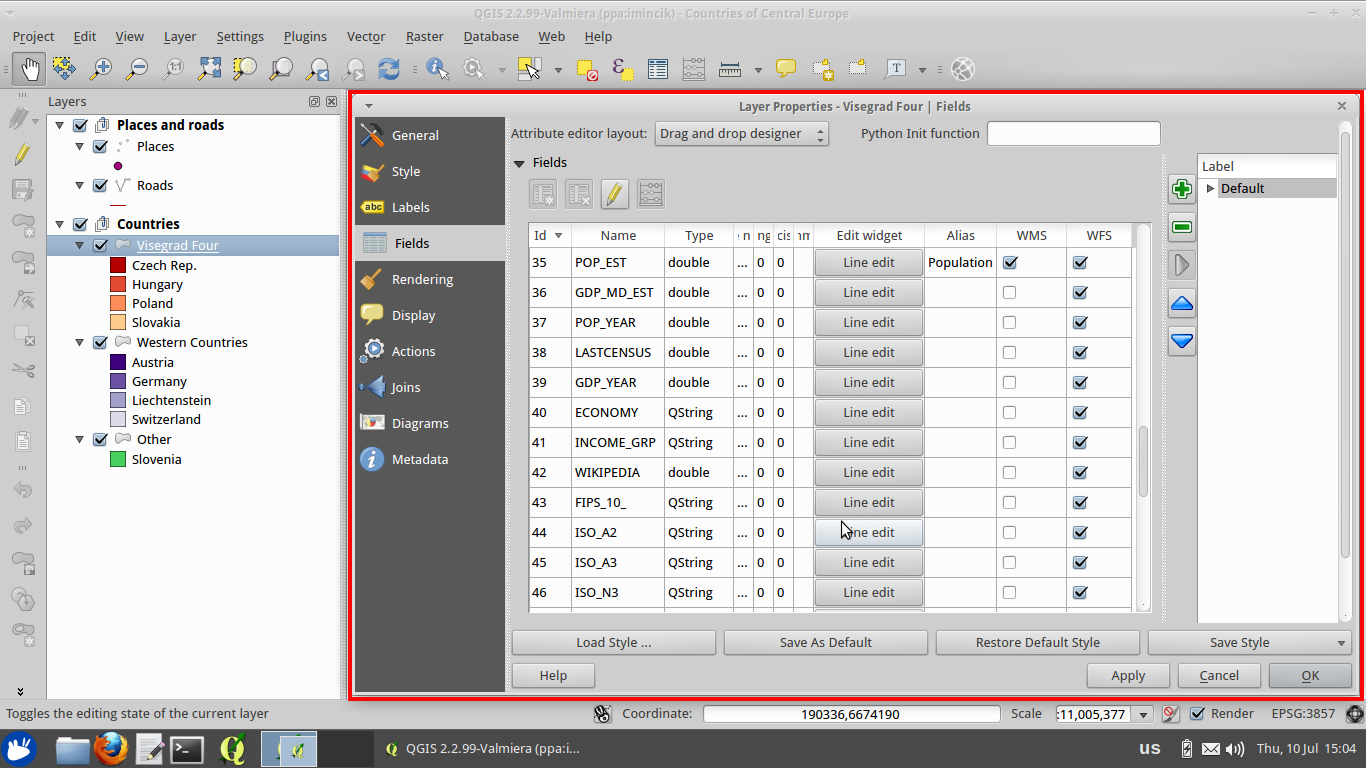
\includegraphics[keepaspectratio=true,height=0.6\textheight]{images/rapid-gis-deployment/project-layer-attributes.png}
	\end{center}
\end{frame}


\begin{frame}{Feature information}
	\begin{itemize}
		\item activate feature info for selected layers
	\end{itemize}
	\begin{center}
		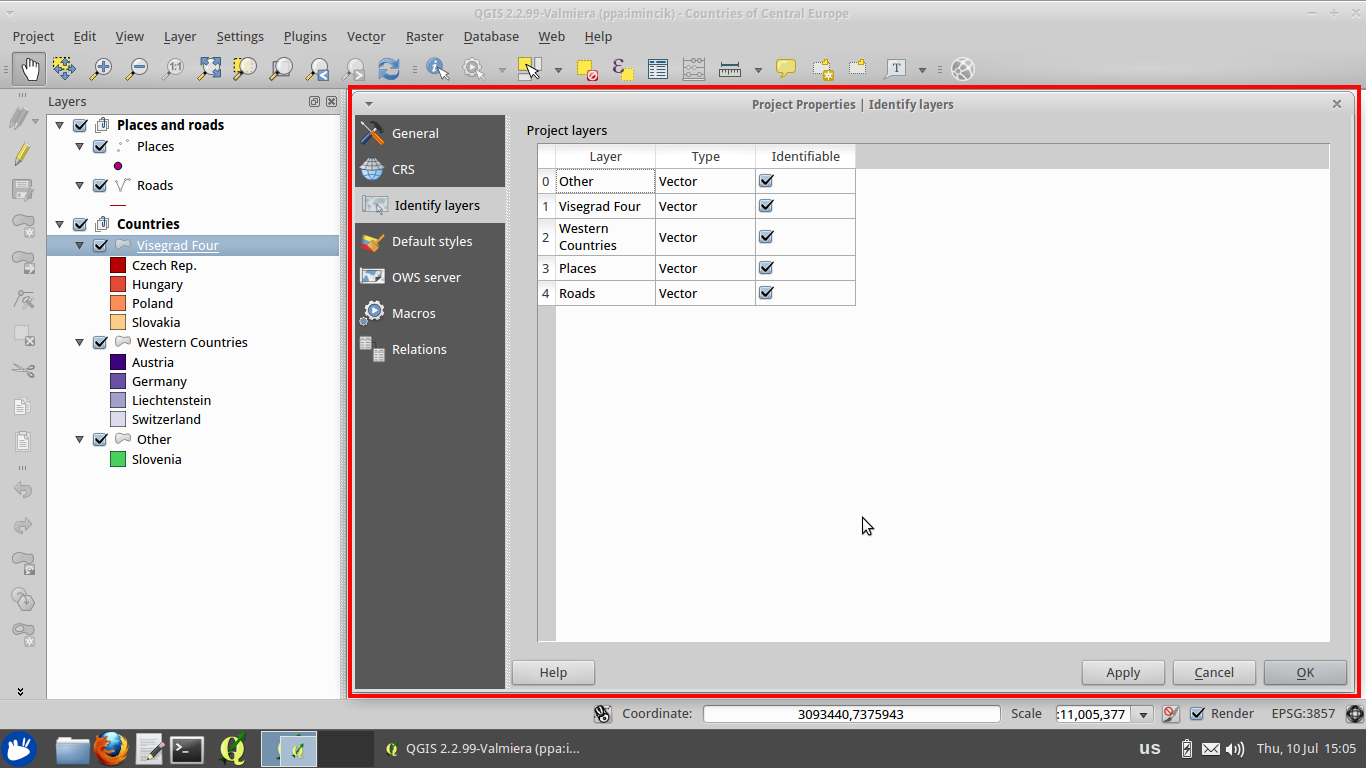
\includegraphics[keepaspectratio=true,height=0.6\textheight]{images/rapid-gis-deployment/project-feature-info.png}
	\end{center}
\end{frame}


\begin{frame}{Project properties}
	\begin{itemize}
		\item set project title, abstract, author name and email
	\end{itemize}
	\begin{center}
		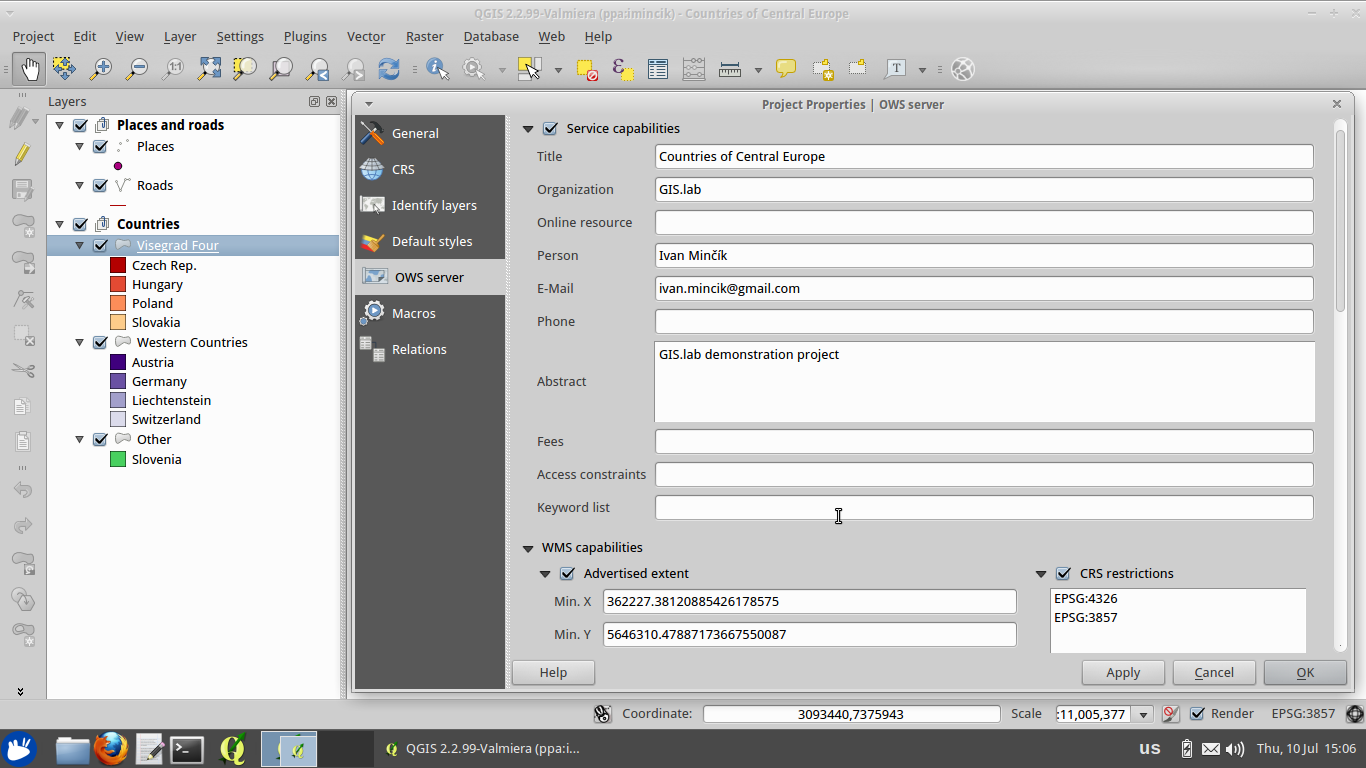
\includegraphics[keepaspectratio=true,height=0.6\textheight]{images/rapid-gis-deployment/project-properties.png}
	\end{center}
\end{frame}


\begin{frame}{Project publishing}
	\begin{itemize}
		\item save project
		\item move project to Share/\$USER directory
	\end{itemize}
	\begin{center}
		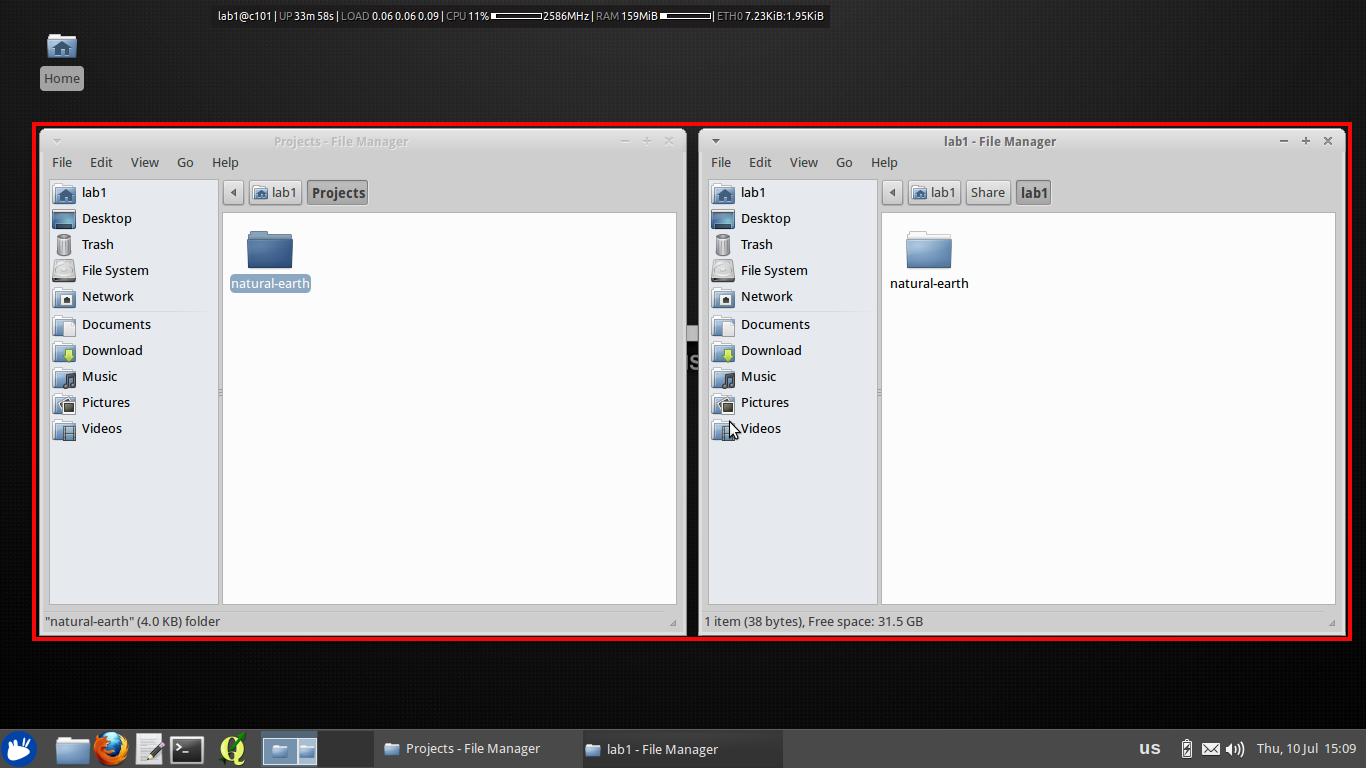
\includegraphics[keepaspectratio=true,height=0.6\textheight]{images/rapid-gis-deployment/project-share-directory.png}
	\end{center}
\end{frame}


\begin{frame}{Project publishing}
	\begin{itemize}
		\item publish project in GIS.lab Web
	\end{itemize}
	\begin{center}
		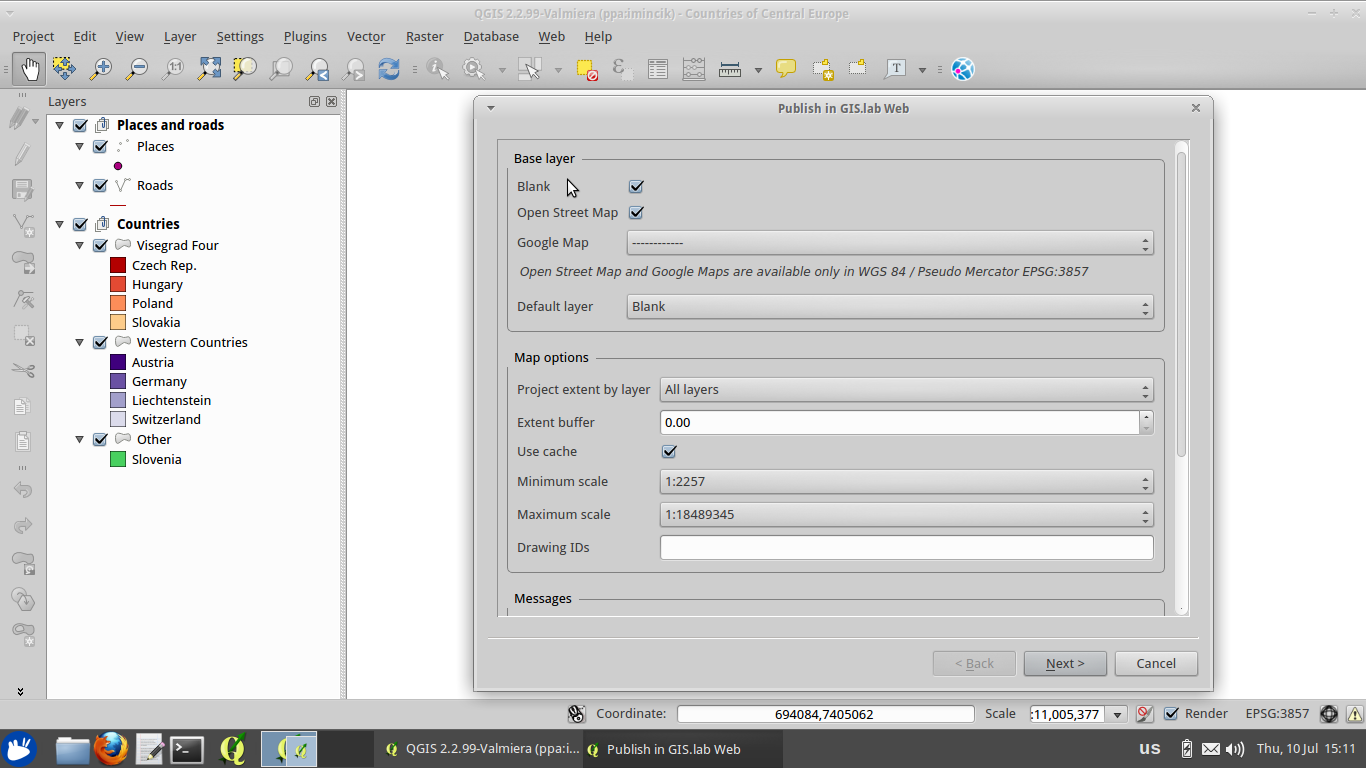
\includegraphics[keepaspectratio=true,height=0.6\textheight]{images/rapid-gis-deployment/project-publish.png}
	\end{center}
\end{frame}


\section{GIS.lab Web}
\begin{frame}
	\begin{center}
		\LARGE\textbf{GIS.lab Web}
	\end{center}
\end{frame}


\begin{frame}{GIS.lab Web}
	\textbf{http://web.gis.lab/?PROJECT=path-to-project}
	\begin{center}
		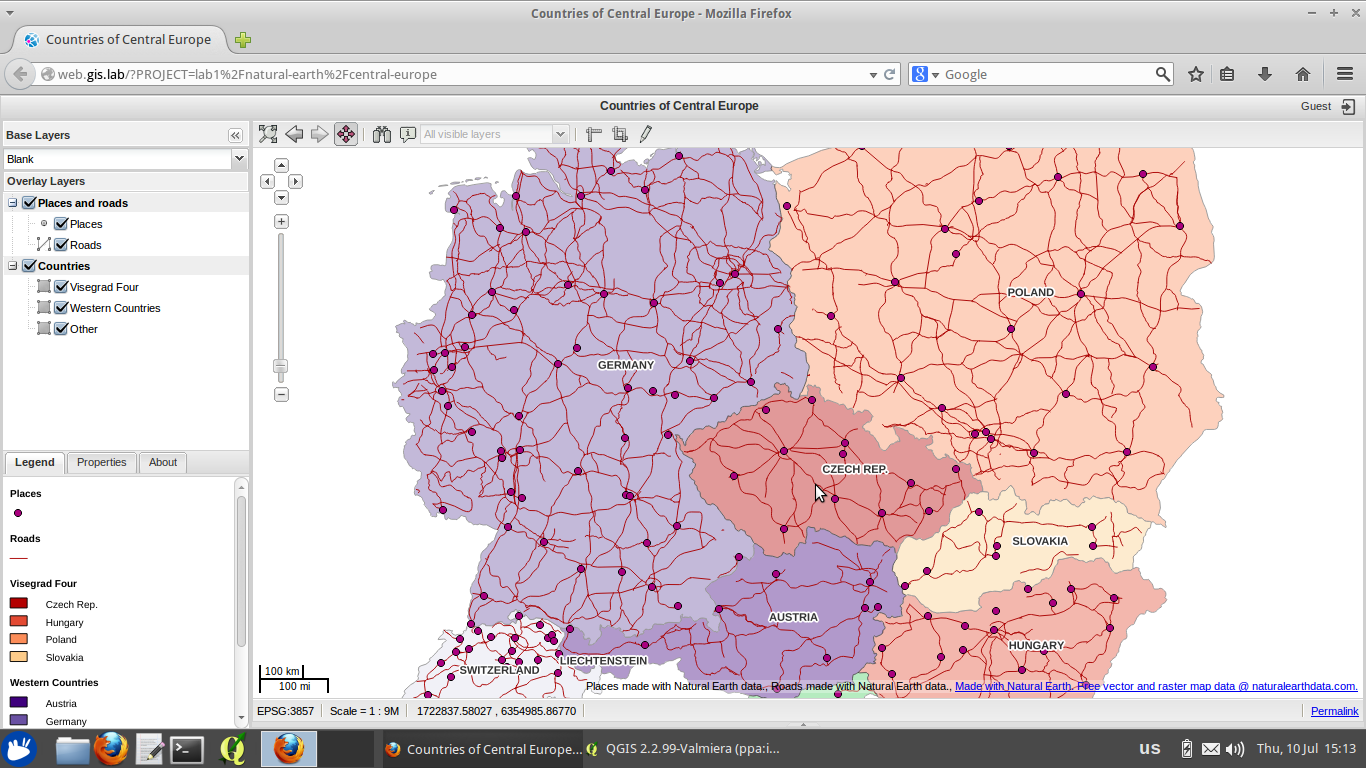
\includegraphics[keepaspectratio=true,height=0.7\textheight]{images/rapid-gis-deployment/project-gislab-web.png}
	\end{center}
\end{frame}


\begin{frame}{GIS.lab Web}
	\begin{itemize}[<+->]
		\item base layers (WMS, OSM, Google), overlay layers from QGIS project
		\item measure lines and polygons
		\item feature information and advanced search
		\item drawing new POINTS, LINES, POLYGONS with attributes
		\item drawing patches to overlay layer's features
		\item print output creation
		\item collaboration tools
		\item high performance, intelligent layers caching
	\end{itemize}
\end{frame}


\begin{frame}{Search in GIS.lab Web}
	\begin{center}
		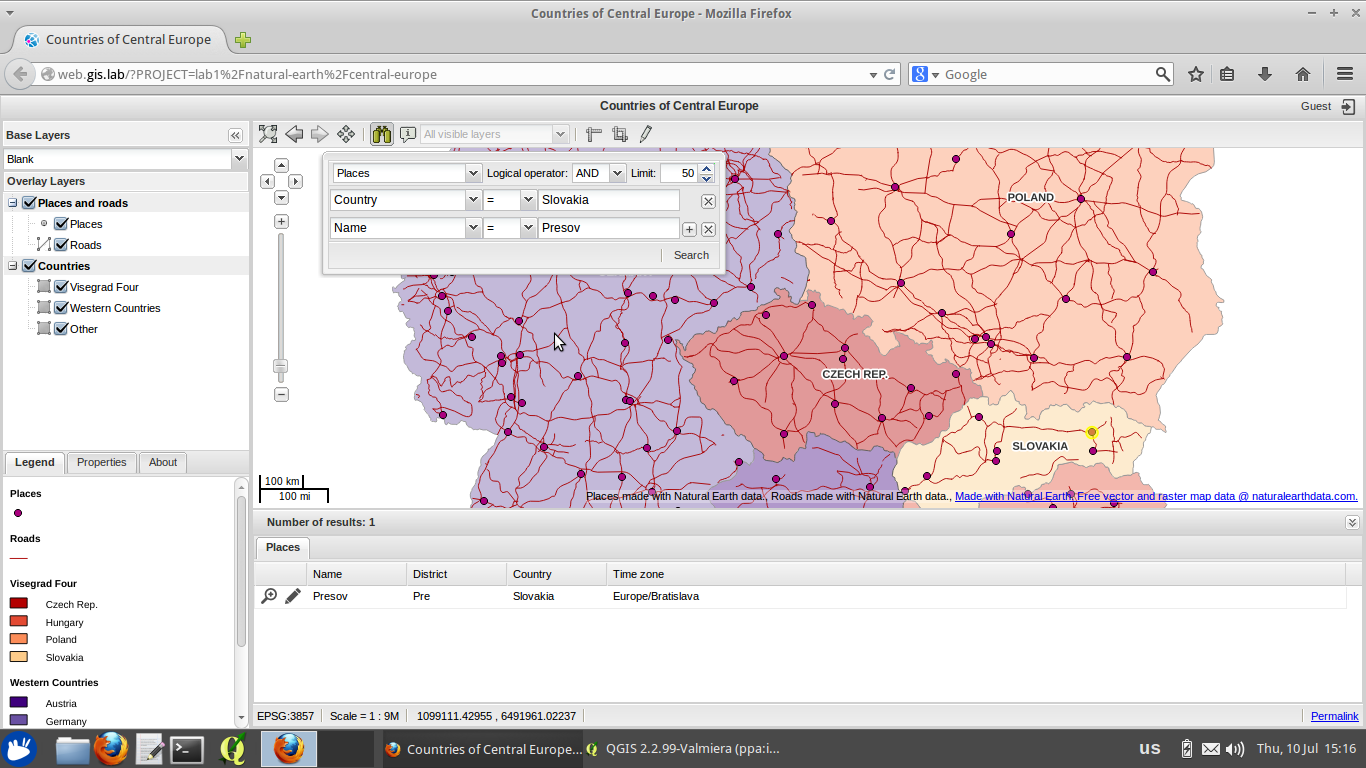
\includegraphics[keepaspectratio=true,height=0.7\textheight]{images/rapid-gis-deployment/project-gislab-web-search.png}
	\end{center}
\end{frame}


\begin{frame}{Drawing in GIS.lab Web}
	\begin{center}
		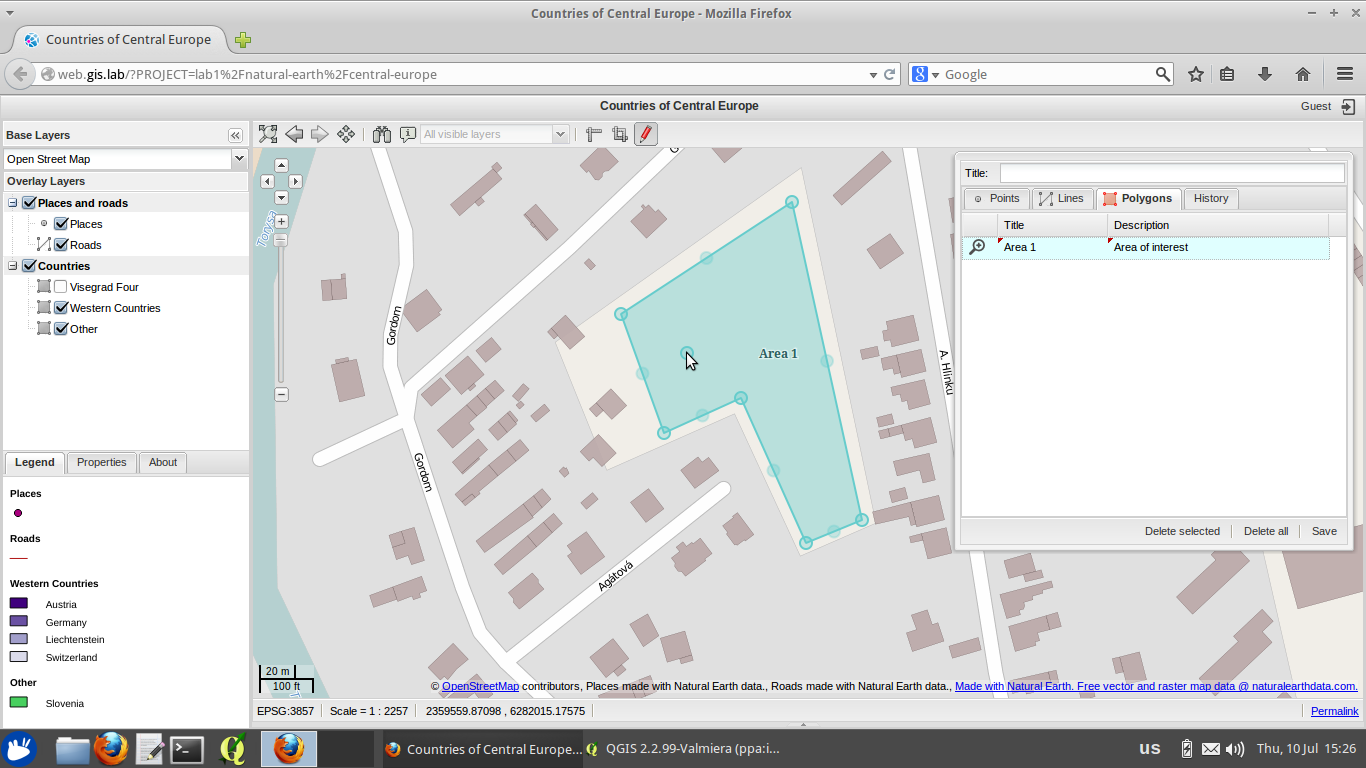
\includegraphics[keepaspectratio=true,height=0.7\textheight]{images/rapid-gis-deployment/project-gislab-web-drawing.png}
	\end{center}
\end{frame}


\section{Amazon AWS}
\begin{frame}
	\begin{center}
		\LARGE\textbf{Amazon AWS provider}
	\end{center}
\end{frame}


\begin{frame}{Installation in Amazon AWS}
	\textbf{Install dependencies}
	\begin{itemize}
		\item \$ vagrant plugin install vagrant-aws
	\end{itemize}

	\textbf{config-user.cfg}
	\begin{itemize}
		\item configure Amazon credentials, placement and security zone
	\end{itemize}

	\textbf{Install GIS.lab server}
	\begin{itemize}
		\item \$ vagrant up --provider=aws
	\end{itemize}
	
	\begin{flushleft}
		\textbf{\textcolor{Cyan}{5} minutes} \\
		\textbf{\textcolor{Cyan}{200} EUR / month} \\
	\end{flushleft}
\end{frame}


\begin{frame}{GIS.lab Web}
	\begin{itemize}
		\item copy project files on AWS server
	\end{itemize}
	\begin{center}
		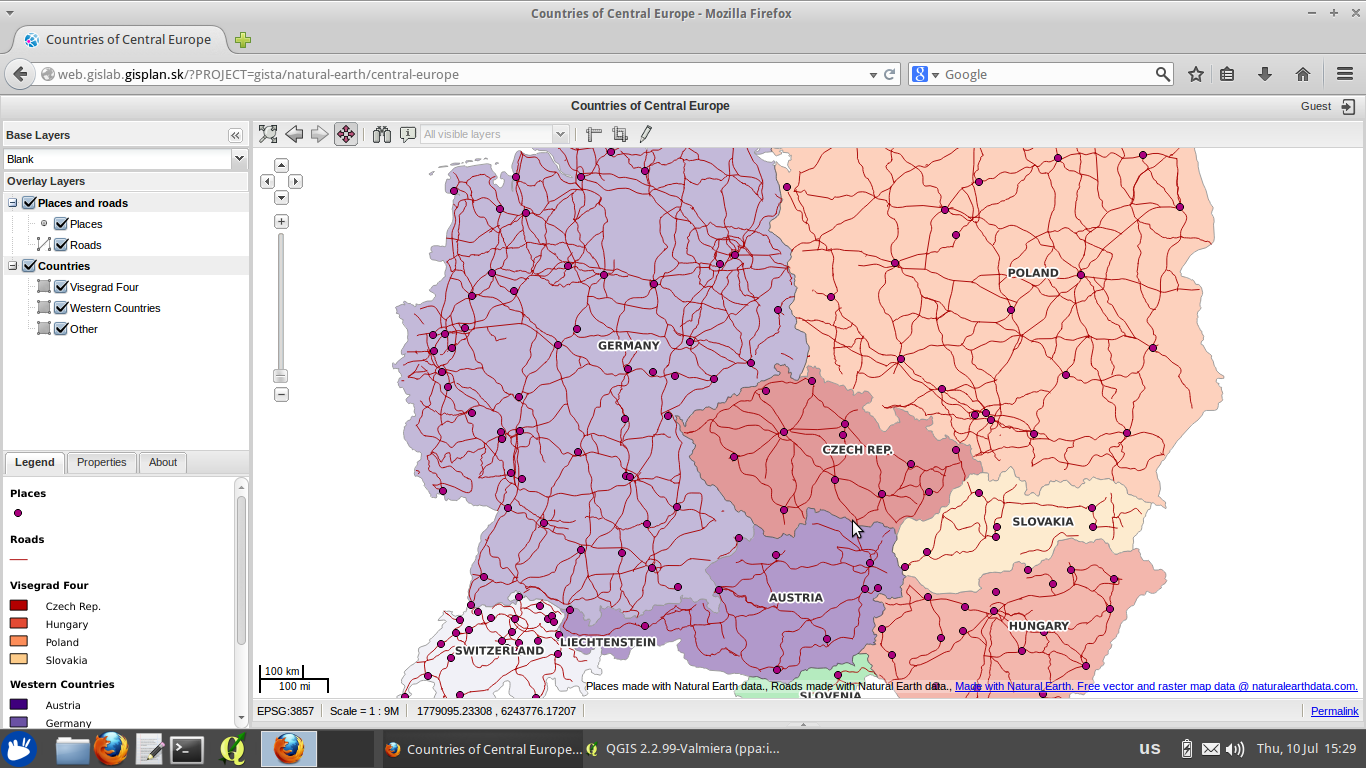
\includegraphics[keepaspectratio=true,height=0.7\textheight]{images/rapid-gis-deployment/project-gislab-web-amazon-aws.png}
	\end{center}
\end{frame}


\section{Future plans}
\begin{frame}
	\begin{center}
		\LARGE\textbf{Future plans}
	\end{center}
\end{frame}


\begin{frame}{Future plans}
	\begin{itemize}
		\item web management interface
		\item multiple templates for GIS.lab Web
		\item deployment changes - use Vagrant and server VM only for local deployment
		\item Docker integration
		\item computing resources sharing between all GIS.lab machines
		\item Web Processing Service (WPS) integration
	\end{itemize}
\end{frame}


\section{Final notes}
\begin{frame}
	\begin{center}
		\LARGE\textbf{Final notes}
	\end{center}
\end{frame}


\begin{frame}{Deployment scenarios}
	\begin{itemize}
		\item virtual client - server infrastructure for local area network (LAN)
		\item GIS server infrastructure in data center or cloud (Amazon Web Services)
		\item development and testing environment
		\item infrastructure for education and Open Source GIS software advocacy
		\item crisis management command center infrastructure (GIS.lab, QGIS, InaSAFE, Ushahidi)
		\item crowd mapping infrastructure
	\end{itemize}
\end{frame}


\begin{frame}{Final notes}
	\begin{itemize}
		\item \textbf{Homepage:} http://imincik.github.io/gis-lab
		\item \textbf{Demo:} http://web.gislab.gisplan.sk/?PROJECT=gista/natural-earth/central-europe
	\end{itemize}
	
	\bigskip
	Thanks for attention.
	
	Ivan Minčík (imincik), ivan.mincik@gmail.com
\end{frame}


% document END
\end{document}